\documentclass[../uwthesis.tex]{subfiles}
\begin{document}

\chapter{Context effects on categorical labeling in children with dyslexia}
\emph{The work below is currently in review at the journal Scientific Studies of Reading as a manuscript with co-authors Liesbeth Gijbels and Jason Yeatman.}

Research shows that on average, children with dyslexia behave less categorically in phoneme labeling tasks. This study investigates three subtle ways struggling readers may perform differently than their typically developing peers in this experimental context: sensitivity to the frequency distribution from which speech tokens are drawn, bias induced by previous stimulus presentations, and fatigue during the course of the task. We replicate findings that reading skill is related to categorical labeling, but we do not find evidence that sensitivity to the stimulus frequency distribution, the influence of previous stimulus presentations, and a measure of task engagement differs in children with dyslexia. It is therefore unlikely that the reliable relationship between reading skill and categorical labeling is attributable to artifacts of the task design, abnormal neural encoding, or executive function. Rather, categorical labeling may index a general feature of linguistic development whose causal relationship to literacy remains to be ascertained. 

\section{Introduction}
It is well established that reading skill is correlated with performance on phoneme categorization tasks, in which listeners are asked to categorize spoken syllables based on a single contrastive phoneme \citep{Noordenbos2015,Vandermosten2010,OBrien2018,OBrien2019CategoricalDuration,Goswami2002}. However, the mechanism underlying the link between impaired processing of phonemes and developmental dyslexia remains unclear. While phonological awareness, the ability to identify and manipulate phonemes, is one of the strongest predictors of dyslexia, there are several reasons to question that phonological processing is the "core deficit" that explains why children with dyslexia struggle learning to read. Some researchers have criticized the "core phonological deficit theory" on the grounds that not enough children could be accurately diagnosed on the basis of phonological awareness alone \citep{Wolf2000Naming-speedHypothesis,Pennington2012IndividualModels.}. Perhaps the most popular line of reasoning, though, is that children with dyslexia perform (on average) poorly on many measures of auditory, visual, working memory, and automaticity that cannot be explained by a phonological deficit alone. These observations have motivated a new wave of research searching for a more fundamental mechanism that might explain the myriad of deficits (including phonological awareness) that are associated with reading (dis)ability.

While some researchers have taken the perspective that individuals with dyslexia have fundamentally impaired auditory or visual processing \citep{Stein2018TheDyslexia,Stein2018TheDyslexia,Goswami2011,Tallal1996}, the psychophysical literature on the whole is currently inconsistent with a uniform pattern of sensory impairment \citep{Hamalainen2013,Amitay2002,Stuart2006,Rosen2003}. Noting this, some researchers have argued that individuals with dyslexia are constrained not by sensory processing at a basic level, but by the demands of psychophysical tasks \citep{Ramus2012,Ahissar2007}. 

While this hypothesis could potentially explain the heterogeneity observed in the sensory processing literature, a consensus is yet to be reached regarding which particular aspects of psychophysical tasks are the "bottleneck" in performance. One candidate is attention and task engagement; dyslexia is comorbid with ADHD \citep{Light1995,Stevenson2005,Germano2010}. In accords with this hypothesis, one previous study has shown that performance on "catch trials" tends to degrade faster over the course of a task in poor readers than controls \citep{Messaoud-Galusi2011} (see also \citep{Roach2004TheDyslexia}). Another candidate is statistical learning. Statistical learning was originally defined as "a way of extracting statistical regularities from the environment" \citep{Saffran1996StatisticalInfants}. It has been proposed that individuals with dyslexia are less able than their typically developing peers to take advantage of regularities in their environment \citep{Banai2006,Ahissar2006,Lieder2019PerceptualDyslexia,Gabay2015}. The statistical learning hypothesis is especially appealing because the process of literacy training involves forming connections between phonological and orthographic representations, which requires a learner to extract regularities from visual and auditory sequences \citep{Ziegler2005ReadingTheory}, and also to learn and automate the probabilistic relationship between a given letter and the phonemes it represents. Thus, there is growing interest in the possibility that individual differences in domain-general mechanisms such as statistical learning could explain degraded performance across an array of experiments as well as a difficulty with learning to read.

The phoneme categorization task is, in some ways, an ideal ground to explore how task performance may be differentially affected by task demands in struggling readers. Because it has been so extensively used, experimenters can have reasonable confidence that the key effect---shallower psychometric functions in struggling readers---is replicable and not specific to a particular acoustic cue \citep{Noordenbos2015,OBrien2018,OBrien2019CategoricalDuration}.

Previously, we showed that reduced categorization in struggling readers is somewhat influenced by the working memory demands of the task, but could not be entirely explained by task difficulty: irrespective of the task-difficulty we found a correlation between reading skill and task performance \citep{OBrien2018}. We now investigate several other aspects of task performance to clarify the extent to which the categorization-reading relationship depends on specific experimental conditions. We first consider the effects of varying the frequency distribution from which speech tokens are drawn. Typically in categorization experiments, stimuli are drawn from a uniform distribution. Distributional learning---sensitivity to the distribution from which stimuli are drawn---is a key part of language acquisition in development \citep{Maye2002InfantDiscrimination}. Neurotypical adults show sensitivity to the stimulus distribution in the categorization task \citep{Clayards2008PerceptionCues}: the task elicits more categorical behavior when stimuli are drawn from narrow bimodal distributions than broad distributions. Recently, work by Vandermosten et al. suggested that children with dyslexia were on average less able to utilize distributional cues to learn a non-native speech contrast \citep{Vandermosten2018StatisticalChildren}. In the present study, we examine how children ages 8-12 performed on a categorical phoneme labeling task with two conditions: a bimodal and uniform distribution of native speech tokens.

Second, we explore how the immediate context of recently presented speech tokens affects judgments about the identity of the current stimulus. Considering how recent stimulus presentations influence performance is of interest for several reasons: it addresses longstanding claims that individuals with dyslexia struggle when stimuli are presented sequentially \citep{Tallal1980} or that they show abnormal stimulus adaptation and faster implicit memory decay \citep{Jaffe-Dax2017DyslexicsAdaptation,Perrachione2016DysfunctionDyslexia,Ahissar2006}. Finally, we look for hallmarks of fatigue and disengagement in our participant's responses by examining changes in task performance over the duration of the experiment. In line with our previous work we find that there is a moderate relationship between phoneme categorization and reading skill; this relationship cannot be attributed to (1) the stimulus distribution, (2) stimulus recency effects or (3) task disengagement. Thus, we conclude that some people with dyslexia have difficulties categorizing speech sounds and that this deficit, though likely not universal, is not an artifact of experimental conditions such as the distribution, order and duration of the experiment.

\section{Methods}
\subsection{Participants}
A total of 62 native English-speaking children ages 8-12 were recruited for the study. Children without known auditory disorders were recruited from a database of volunteers in the Seattle area (University of Washington Reading \& Dyslexia Research Database; https://ReadingAndDyslexia.com). Parents and/or legal guardians of all participants provided written informed consent under the University of Washington Institutional Review Board protocol. All subjects demonstrated normal or corrected-to-normal vision. Participants were tested on a battery of cognitive and literacy assessments, including the Woodcock-Johnson IV (WJ-IV) Letter-Word Identification and Word Attack subtests, the Test of Word Reading Efficiency (TOWRE), and the Weschler Abbreviated Scale of Intelligence. All participants underwent a hearing screening to ensure pure tone detection at octave frequencies between 500 Hz and 8000 Hz in both ears at 25 dB HL or better.


\subsection{Demographics}

Here, we present analyses of task performance where reading skill is treated as either a continuous or discrete group variable. We have previously argued that reading skill is best modeled as a continuous variable, in agreement with Shaywitz et al. that there is no clear demarcation between readers who are below-average and readers who are dyslexic \citep{Shaywitz1992EvidenceAbility}. Our results on phoneme categorization published thus far \citep{OBrien2018,OBrien2019CategoricalDuration}confirm an entirely continuous relationship between task performance and reading skill. However, for completeness and ease of comparison with existing literature on dyslexia, we also provide group-level analyses.  

Reading skill was summarised in a composite variable: as both the WJ-BRS and the TOWRE index are scored on the same standardized scale, a composite reading skill measure was created by averaging the two metrics for each participant. Using a composite of both measures as our criterion improved the confidence of our group assignments since they are highly correlated measures in our sample ($r=0.877, p<2e-16$). Participants were assigned to the Dyslexia group if their composite reading score was at least 1 standard deviation below the population mean (i.e., $<85$). No participant in the Control group had any parental report of dyslexia or a history of reading disability. All subjects were required to have nonverbal IQ and full-scale IQ (WASI Matrix Reasoning and FS-2 scores respectively) no less than 1 standard deviation below the population mean (as in \citep{OBrien2018,OBrien2019CategoricalDuration}); 3 subjects were below this cutoff and excluded from further analysis. 

There were 24 subjects in the Dyslexic group (13 male) and 35 subjects in the Control group (16 male). There was not a significant difference in age between groups (Kruskal-Wallis rank sum test, $H(1)=2.194, p=0.139$), although we noted that there was a small correlation between age and reading skill ($r = 0.253, p = 0.053$). Importantly, we included age as a covariate in our analyses. We did not exclude participants with ADHD diagnoses from the study because ADHD is highly comorbid with dyslexia [Germano et al 2010]. Instead, we accounted for ADHD diagnosis as a covariate in our statistical analyses. Of 59 participants, 13 had a formal diagnosis of ADHD: 7 in the Dyslexic group and 6 in the Control group. The difference in prevalence of ADHD across groups was not significant ($H(1) = 1.178, p=0.278$).

Table ~\ref{tab:group_demo} shows group comparisons on measures of reading and cognitive skills. As in our previous findings, IQ (either measured as full-scale or nonverbal) differed by group. While we were not concerned that low IQ prevented any subject from understanding the task because low IQ was an exclusion criterion, we included nonverbal IQ as a covariate in our statistical analyses. 

\begin{table}
  \begin{threeparttable}
    \caption{Summary statistics and group differences on demographic and behavioral measures.}
    \label{tab:group_demo}
    \begin{tabular}{llll}
    \toprule
      & Control & Dyslexic & Significance\\
    \midrule
     & $n=$35 & $n=$24 & \\
     & 16 male, 19 female & 13 male, 11 female & \\
    \textbf{WASI-III} &  &  & \\
    FS-2 & 121 (12.7) & 101.8 (13.1) & $<$ 0.001\\
    Nonverbal IQ & 59.6 (8.7) & 50.3 (7.8) & $<$ 0.001\\
    \textbf{Woodcock-Johnson IV} &  &  & \\
    Basic Reading Score & 111.6 (12.1) & 79.8 (7.2) & $<$ 0.001\\
    Nonword & 111.3 (13.5) & 87.8 (10) & $<$ 0.001\\
    Real Word & 110.4 (11.6) & 74.8 (10.3) & $<$ 0.001\\
    \textbf{TOWRE 2} &  &  & \\
    TOWRE Index & 101.7 (12.8) & 69.5 (7) & $<$ 0.001\\
    Nonword & 100.5 (14.8) & 72.9 (8.2) & $<$ 0.001\\
    Real Word & 102.8 (12.3) & 69.2 (9.3) & $<$ 0.001\\
    \textbf{CTOPP 2} &  &  & \\
    Phonological Awareness & 101 (13.8) & 91.6 (11.4) & 0.021\\
    Phonological Memory & 99.1 (13.7) & 88.2 (12.1) & 0.003\\
    Rapid Naming & 98.7 (11.2) & 83.7 (9.8) & $<$ 0.001\\
    \bottomrule
\end{tabular}
    \end{threeparttable}
\end{table}


\subsection{Stimuli}
A 7-step /ba/$\sim$/da/ speech continua were created using Praat v. 6.0.37. In the /ba/$\sim$/da/ continuum, the starting frequency of the second vowel formant (F2) transition was varied. Note that this is the same continuum used in \citep{OBrien2019CategoricalDuration}, to which we refer the reader for greater detail on the synthesis procedure. In brief, the seven speech tokens were identical except for their F2 formant contour. The starting frequency of F2 was varied in seven linearly-spaced steps from 1085 Hz (/ba/) to 1460 Hz (/da/). F2 rose in a linear ramp to a terminal value of 1225 Hz over the course of 100 ms, at which point the steady-state portion of the vowel was maintained for 250 ms. 

\subsection{Procedure}
Stimulus presentation and participant response collection was managed with PsychToolbox for MATLAB \citep{Brainard1997}. Auditory stimuli were presented at 75 dB SPL via circumaural headphones (Sennheiser HD 600). Children were trained to associate sounds from the two speech continua with animal cartoons on the left and right sides of the screen and to indicate their answers with right or left arrow keypresses. Large text labels were provided over each animal cartoon ("Ba" on the left side and "Da" on the right), so participants did not have to memorize the animal associated with each sound. Throughout all blocks, each cartoon was always associated with the same stimulus endpoint.

Participants first completed a practice round consisting of ten presentations, five of each continuum endpoint, with feedback on each trial. Participants were allowed to repeat the practice round up to three times, until they had achieved at least 75\% accuracy. All participants were able to meet this minimum standard.

The main task was presented in two parts, one in which the stimuli were drawn from a uniform frequency distribution and another in which they were drawn from a bimodal distribution. In the unimodal condition, all stimuli were presented 15 times. In the bimodal condition, the presentation frequency was greatest at the continuum endpoints and least in the center of the continuum (see Table~\ref{tab:stim_freq}).  

Because we were interested in exploring the effects of recently presented stimuli on judgments about the current stimulus, we used a "random but frozen" list of stimuli. This means that we randomly generated the order in which stimuli would be presented in each condition, but every participant was tested with this fixed stimulus order. This reduced one source of variability across subjects so that we could perform more targeted investigations about how recent stimulus presentations differentially affect strong and poor readers.

\begin{table}
    \caption{Stimulus presentation frequency in bimodal condition.}
    \label{tab:stim_freq}
    \centering
        \begin{tabular}{llllllll}
        \toprule
        \textbf{Stimulus} & 1 & 2 & 3 & 4 & 5 & 6 & 7\\
        \midrule
        \textbf{Frequency} & 52 & 34 & 14 & 10 & 14 & 34 & 52\\
        \bottomrule
        \end{tabular}
\end{table}

In each condition (uniform or bimodal frequency distribution), participants heard a total of 210 speech sounds. After every 35 stimulus presentations, a quick optional break was presented. Between the two test conditions, reading assessments were performed. If a participant did not already have an IQ measure on file from a previous lab meeting, the WASI-III was also administered.

Seven participants completed the uniform condition first and 45 completed the bimodal condition first. The reason for this discrepancy is that during data collection for the first 15 subjects, we alternated which condition was presented first. After data was collected for these subjects, we were surprised to see little evidence that participants behaved differently in either condition. We therefore changed to a policy of always providing the bimodal condition first, wary that initial exposure to the uniform condition could affect category learning in subsequent conditions. We considered simply discarding the data of the seven subjects who performed the uniform condition first; however, we were unable to detect any significant differences between task performance in these individuals and the remainder of the cohort. Psychometric function slope did not significantly differ by group ($\beta = -0.140$, SE = 0.331, $p=0.674$), nor was there a significant interaction between the order conditions were presented and slope in each condition ($\beta = -0.0715$, SE = 0.309, $p=0.818$). On this evidence, we retained these seven subjects in the data set, although they are clearly marked so any analyses can be re-run with or without them present. 

\subsection{Psychometric curve fitting}
As in all previous chapters, we used the MATLAB toolbox Psignifit 4.0 to fit psychometric functions. The fitting routine optimized the fit of a logistic curve function with four parameters modeling the upper and lower asymptotes, width of the logistic function, and the threshold. The width of the logistic function was transformed to the slope at the threshold value to give a standardized measure of psychometric function slope. 

Psignifit uses a Bayesian framework to optimize parameter estimates not only according to likelihood of generating a given set of behavioral responses, but also with regard to prior distributions of each parameter. In the case of psychometric function fitting, where the number of presentations of each stimulus is often relatively low, inappropriate priors can have an outsized influence on parameter estimates- particularly, as we and many others have summarized elsewhere, when it comes to estimates of the slope and asymptotes. We therefore used priors validated in our previous work on a similar task, with a similar participant demographic \citep{OBrien2019CategoricalDuration}: the asymptotic priors were modeled as a uniform distribution on the range [0, .10]. In other words, the lower and upper asymptotic parameters could vary freely in the range [0, .10], to give a lower asymptote between 0-10\% and an upper asymptote between 90-100\%. This prior width was chosen on the basis of ten-fold cross-validation over the dataset (see \citep{OBrien2018,OBrien2019CategoricalDuration} for further details). 

To ensure the validity of psychometric function parameter estimates, as in our previous work \citep{OBrien2018,OBrien2019CategoricalDuration} we excluded any psychometric functions that could not be fit with a threshold between continuum steps 1 through 7. Only one psychometric function (produced by a subject in the Dyslexic group presented with a uniform stimulus distribution) was excluded on this ground. 


\subsection{Statistical analysis of parameter estimates}
After we fit psychometric functions for each subject in each condition, we used a series of generalized linear mixed models to determine the relationship between reading ability, the frequency distribution from which stimuli are drawn, and three dependent measures. As in \citep{OBrien2018,OBrien2019CategoricalDuration},these dependent measures were estimates of task performance based on behavioral responses: (1) psychometric function slope, (2) lapse rate, and (3) a composite measure of psychometric function shape. 

Lapse rate was determined by averaging the upper and lower asymptote estimates of a given function (i.e., their deviations from 0 and 1 respectively). The composite measure was constructed from a principal components analysis on the four parameters of each psychometric function collected in the study. The first principal component captured 45.5\% of variance in the four parameters, and was defined by the following linear weights: threshold: -0.385, slope: 0.486, upper asymptote: -0.498, lower asymptote: -0.606. 

Model selection was performed using the \texttt{lme4} library for R with parametric bootstrapping tests of model fit performed with the \texttt{pbkrtest} library. For each dependent measure, fixed-effect predictors with sum coding were used for the condition (uniform or bimodal) variable. Reading ability was entered as a continuous fixed-effect predictor except where otherwise stated. Additional predictors were added for presence/absence of ADHD diagnosis (treatment coding), age (continuous predictor) and for non-verbal IQ (WASI-III Matrix Reasoning score; continuous predictor). A random intercept for participant was also included. For all model analyses, we began with a fully specified model of reading score as a function of the parameters of interest (slope, asymptote, or PC1) plus the covariates (ADHD, age and non-verbal IQ) and a random intercept for subject identity. The contributions of the covariates were first tested using parametric bootstrapping, which is robust to non-normally distributed residuals. Model terms were retained if the bootstrapped p-value of the coefficient being nonzero was less than 0.1. After testing the three covariates, we tested terms of interest for the study (condition, reading ability, and the interaction between them) using the same procedure.

\section{Results}
 
 As expected on the basis of previous studies in our lab and others, we found relationships between reading skill and psychometric function shape \citep{OBrien2018,OBrien2019CategoricalDuration,Vandermosten2010,Noordenbos2015}. In Figure ~\ref{fig:reading_par}, we can see that psychometric slope, asymptote and PC1 (a general measure of psychometric function shape) were all correlated with reading ability. 
 
 
 \begin{figure}
    \centering
    \caption{Relationship between reading skill and phoneme categorization.}
    \label{fig:reading_par}
    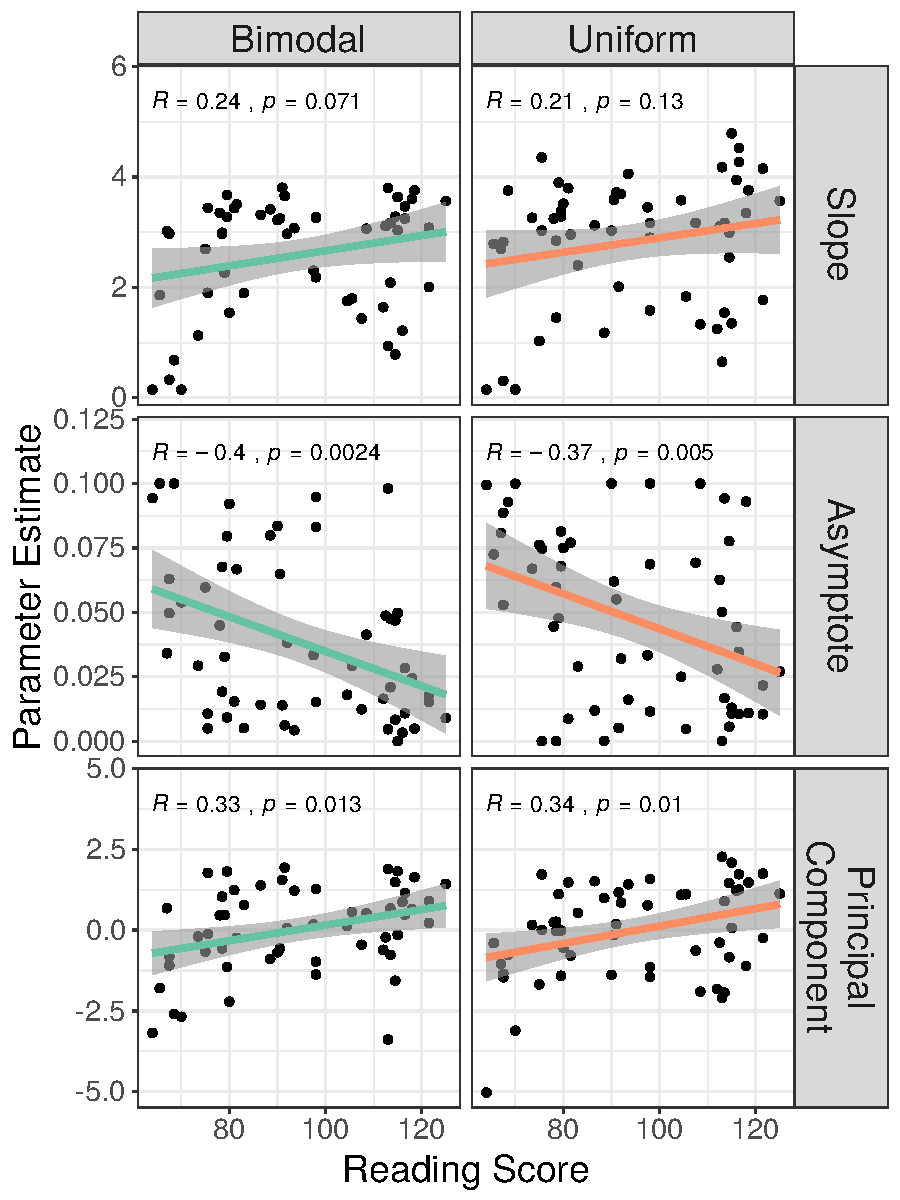
\includegraphics[width = 10 cm]{images/paper_4/parameter_relationships.pdf}
    \item \textit{Plots of model psychometric function parameter estimates versus reading score. Each point corresponds to parameter estimates for one subject in one condition (bimodal or uniform). Lines indicate the best fit regression line with 95\% confidence intervals in shaded regions.}
\end{figure}
 
We confirmed this with generalized linear mixed model analysis, first with regard to the relationship between reading ability and psychometric slope. After model selection, the most parsimonious model of psychometric slope contained a continuous predictor for reading ability only (Table ~\ref{tab:psy_models}).
 
Note that in addition to the covariates (age, ADHD diagnosis, and nonverbal IQ), the main effect  of condition ($\beta = 0.265$, SE = 0.162,$p=0.107$) and the interaction between condition and reading ability ($\beta = -0.061$, SE = 0.163,$p=0.708$) were dropped by model selection. Thus, we did not detect a significant relationship between psychometric slope and the frequency distribution from which stimuli were drawn. Moreover, we did not find evidence supporting the hypothesized interaction between reading skill and experimental condition (bimodal or uniform). In other words, we replicate the equivalent relationship between phoneme categoriztion and reading skill irrespective of the distribution from which the stimuli were drawn.
 

Similarly, the selected model of lapse contained only main effects of reading skill and the covariate, age (Table~\ref{tab:psy_models}). Lastly, considering PC1 as the dependent variable, the selected model contained only main effects of reading skill and age (Table~\ref{tab:psy_models}). Taken as a whole, no aspect of psychometric shape appears to depend on the task condition for strong or struggling readers. 

% Lapse
\begin{table}[ht]
\centering
\caption{Selected models of psychometric function parameters}
\label{tab:psy_models}
\begin{tabular}{llrrl}
\toprule
  & & $\beta$ & SE & $p$\\
\midrule
\textbf{Slope} \\
& (Intercept) & 2.723 & 0.12 & $<$ 0.001\\
& Reading skill & 0.223 & 0.12 & 0.069\\
\midrule
\textbf{Lapse} \\
& (Intercept) & 0.102 & 0.023 & $<$ 0.001\\
& Reading skill & -0.010 & 0.003 & 0.006\\
& Age & -0.006 & 0.002 & 0.013\\
\midrule
\textbf{PC1}
&(Intercept) & -2.777 & 1.111 & 0.016\\
&Reading skill & 0.342 & 0.162 & 0.039\\
&Age & 0.279 & 0.111 & 0.015\\
\bottomrule
\end{tabular}
\end{table}




For completeness, we also tested the interaction of reading skill and stimulus distribution with reading skill treated as a categorical variable (Dyslexic vs. Control). A mixed effects ANOVA with a random effect of subject was used to evaluate the interaction term, using the Kenwards-Rogers estimation of degrees of freedom. The interaction was not significant in a model of slope ($F(1,55.6) = 0.860, p = 0.357$), lapse ($F(1,61.7)= 0.390, p = 0.535$), or PC1 ($F(1,53.3) = 0.390, p = 0.861$). The estimated Cohen’s $d$ for the separation of slope by group was 0.48, with a 95\% confidence interval ranging from -0.09 to 1.04; this range is consistent with results in two of our previous studies and the average effect size in a meta-analysis of categorical labeling studies \citep{OBrien2018,OBrien2019CategoricalDuration, Noordenbos2015}. For separation of lapse by group, $d=0.75$ (CI $= [0.17,1.32]$), and for separation of PC1 by group, $d=0.64$ (CI $= [0.07,1.20]$).

Altogether, our analyses indicate that from the behavioral responses alone, there was no evidence for sensitivity to the stimulus distribution in our sample of participants. This makes it challenging to interpret our data as evidence for or against a statistical learning deficit in struggling readers. What our data do suggest is that the apparent relationship between reading skill and performance on the categorical phoneme labeling task is not likely to be a simple artifact of the stimulus frequency distribution chosen by the experimenter. 

\subsection{Effects of recent stimulus presentations on phoneme labeling}
Because we collected 420 responses per individual, our dataset may provide sufficient power to examine stimulus recency effects. To explore this possibility, we employed the modeling approach of Lieder et al. \citep{Lieder2019PerceptualDyslexia}, which uses generalized linear models to investigate how recent stimulus presentations affect the judgment of the current stimulus' identity. 

For every stimulus presentation in the data set, we determined the identity of the preceding four stimuli. As in \citep{Lieder2019PerceptualDyslexia}, we adopt the following notation:

Let $d_0$ be the stimulus step (1-7) of the current stimulus presentation, $t$. Then $d_1$ is the difference in steps between $d_0$ and the stimulus presented at trial $t-1$. Similarly, $d_2$ is the difference in steps between $d_0$ and the stimulus presented at trial $t-2$, and so on for values $d_3$ and $d_4$.

The mixed effects GLM specifying the relationship between the label assigned to the current stimulus presentation and the recent presentations is as follows:
\begin{equation}
\label{eqn:GLM}
\centering
response = f(\beta_0 + \beta_1d_0 + \beta_2d_1 + \beta_3d_2 + \beta_4d_3 + \beta_5d_4 + (1|Subject ID))
\end{equation}

where $f$ is the probit link function, $\beta$ coefficients are linear weights to be estimated, $d_0$ represents the continuum step of the current stimulus presentation, and $(1|Subject ID)$ is a random intercept for subject. The probit was chosen as the link function because the dependent variable, $response$, is binomially distributed--i.e., participants decided whether a sound was "da" or not. We note that the probit function contains only two parameters that variously adjust the slope and threshold of a sigmoid, and, therefore, attentional lapses would have an effect the estimated slope. 

For the purpose of illustrating this approach clearly, we begin with an exploration of group differences and then move on to a model where reading skill is treated as a continuous variable. We first fit a mixed effects GLM to the responses of each group (Control and Dyslexic). The estimated coefficients are compared in Figure~\ref{fig:recency_fx_group}.

 \begin{figure}
    \centering
    \caption{Estimates of recency effects in Control and Dyslexic groups.}
    \label{fig:recency_fx_group}
    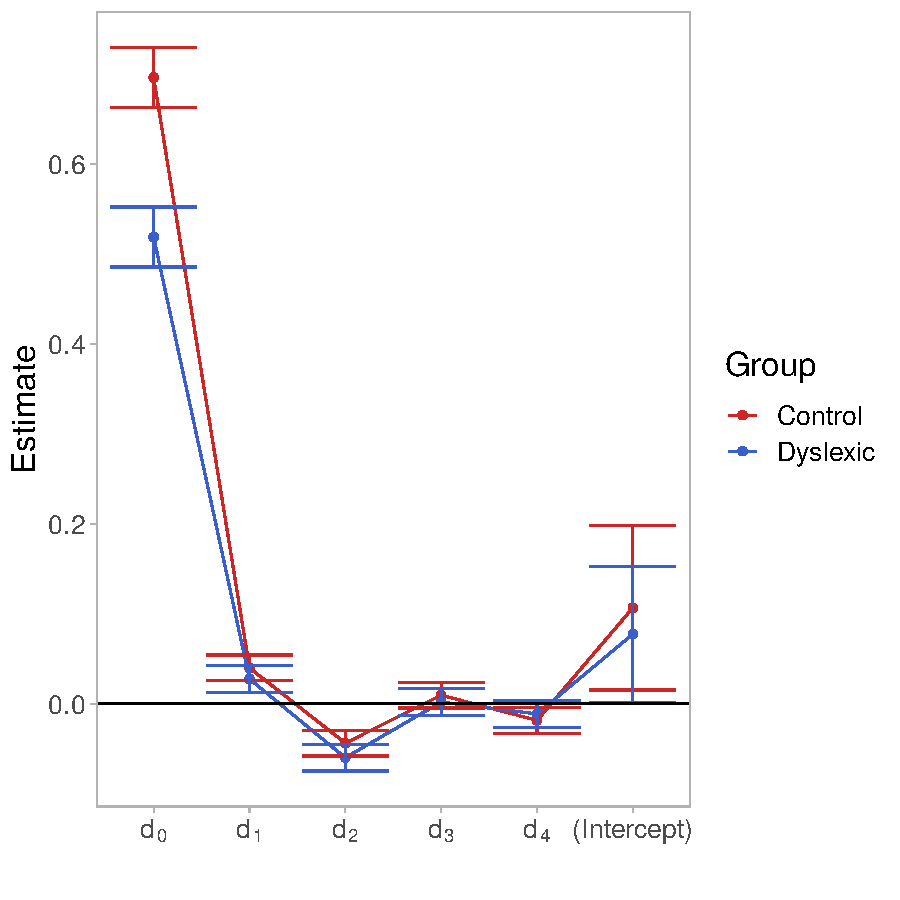
\includegraphics[width = 10 cm]{images/figure_4/recency_fx_group.pdf}
    \item \textit{Estimates of coefficients from a mixed effects generalized linear model (GLM) fit to group behavioral data. Bars indicate the 95\% confidence interval surrounding a given estimate.}
\end{figure}
 
We can immediately see that stimulus recency effects exist and ($d_1$ through $d_4$) are quite similar between groups. The coefficient that differs by group is the weighting of $d_0$---in other words, the mixed effects GLM estimates that probit slope is lower in the Dyslexic group even when recent stimulus presentations are accounted for. The intercept term, which quantifies the threshold of the probit function, is non-zero (i.e., the threshold is not exactly at the center of the continuum) but appears not to differ meaningfully by group. 

Having visualized the group-level differences, we follow up with a treatment of reading skill as a continuous measure in the GLM. On the basis of our initial exploration, we drop the terms $d_3$ and $d_4$ from the model, as the standard errors for these point estimates suggests we are under-powered to detect recency effects at this timescale. 

First, we consider the mixed effects GLM containing main effects of $d_1$, $d_2$, $d_0$ and reading skill, plus an interaction of $d_0$ and reading skill. We hypothesized a significant interaction between reading skill and $d_0$ on the basis of the previous group-level model. Indeed, the interaction as well as the stimulus recency terms were all highly significant (Table~\ref{tab:GLM_model}). 

\begin{table}
\centering
\caption{Hypothesized model of behavioral response} \label{tab:GLM_model}
    \begin{tabular}{lrrl}
    \toprule
      & $\beta$ & SE & $p$\\
    \midrule
    (Intercept) & 0.097 & 0.034 & 0.005\\
    $d_{inf}$ & 0.634 & 0.010 & $<$ 0.001\\
    Reading skill & 0.002 & 0.034 & 0.95\\
    $d_1$ & 0.034 & 0.005 & $<$ 0.001\\
    $d_2$ & -0.049 & 0.005 & $<$ 0.001\\
    $d_{0}*$Reading skill & 0.133 & 0.006 & $<$ 0.001\\
    \bottomrule
    \end{tabular}
\end{table}

We also tested augmenting our hypothesized model to include an interaction between reading skill and stimulus recency terms $d_1$ and $d_2$. Adding a $d_1*$Reading skill interaction increased the AIC from 15604.6 to 15604.8 and the BIC from 15660.7 to 15668.8, and the new interaction term was not significant ($\beta = 0.007$, SE = 0.005, $p= 0.184$).  Considering a $d_2$*Reading skill interaction term fared no better: the interaction was not significant ($\beta = 0.0007$, SE = 0.005, $p=0.894$), and AIC and BIC increased (to 15606.5 and 15670.7 respectively) compared to the simpler model. 

From this investigation of stimulus recency effects, we find that we are able to detect significant effects of the last two stimulus presentations on judgments of the current stimulus' identity. Our models do not provide evidence for an interaction of reading skill and the influence of previous stimulus presentations. Rather, the model upholds the interpretation that psychometric functions are steeper in stronger readers, regardless of the context each stimulus presentation occurs in.  

Lastly, we performed an analysis to characterize the mechanism by which recently presented stimuli influence judgments of the current stimulus. We hypothesized that if the current stimulus was ambiguous---i.e., it was drawn from the center of the /ba/$\sim$/da/ continuum---then the influence of the previous stimulus would be greatest. In other words, listeners might make greater use of the contrast between the current and previous stimuli when the current stimulus is ambiguous than when thee current stimulus is a clear category exemplar. We tested this hypothesis with another mixed effects GLM. First, we created a new binary feature that distinguishes stimuli drawn from the center of the continuum versus the endpoints:

\[
    ambiguous =
    \begin{cases}
        0 & \text{if $d_0 \in$ [Steps 1,2,6,7],}\\
        1 & \text{otherwise.}
    \end{cases}
\]


We then tested the model

\begin{equation}
\centering
response = f(\beta_0 + \beta_1d_0 + \beta_2d_1*ambiguous + (1|Subject ID))
\end{equation}

where $f$ is a probit function as in Eqn.~\ref{eqn:GLM}. We were specifically interested in the interaction of $d_1$ and $ambiguous$: a significant interaction indicates that magnitude of the difference between the current and past stimulus depends on whether the current stimulus is a category exemplar or not. As expected, the interaction of $d_1$ and $ambiguous$ was significant ($\beta=0.085$, SE $=0.007,p<0.001$). This analysis upholds the intuition that previous trials influence the present judgment by providing a contrast to judge ambiguous stimuli by. If this is indeed the primary mechanism by which stimulus recency effects influence performance on the categorization task, then our study is not alone in finding a lack of interaction between reading skill and such contextual effects: Blomert et al. \citep{Blomert2004} also found no evidence for context effects at several linguistic scales in a phoneme labeling task like ours.


\subsection{Quantifying fatigue during the task}
The relatively large number of trials collected per subject allows us to revisit an analysis proposed by Messaoud-Galusi et al. \citep{Messaoud-Galusi2011}, to determine whether poor readers show precipitous declines in task performance as the study goes on. If poor readers become fatigued or distracted at a faster rate than strong readers, that could explain overall differences in task performance. 

To this end, we modeled the probability of correctly labeling a clear "ba" or "da" exemplar as a function of trial number and reading skill. Note that clear category exemplars are stimuli drawn from the two ends of the continuum (steps 1 and 7). Having already established that poor readers produce shallower psychometric functions overall, we should expect that the probability of correctly labeling these tokens will be lower overall in poor readers. If an interaction of trial number and reading skill is found to be significant, that would suggest task fatigue occurs differentially across the spectrum of reading skill. 

Once again, we used a mixed effects GLM with subject as a random effect (as each subject participated in two test conditions, each with 210 trials). The dependent variable was accuracy on labeling an endpoint of the continuum, which was coded as 1 or 0. The model included a main effect of trial number, a main effect of reading skill, and an interaction of the two. Trial number and reading skill were scaled and centered prior to modeling. The results of this analysis are provided in Table~\ref{tab:fatigue}.

\begin{table}
\centering
\caption{Model of accuracy labeling continuum endpoints} \label{tab:fatigue}
    \begin{tabular}{lrrl}
    \toprule
      & $\beta$ & SE & $p$\\
    \midrule
    (Intercept) & 1.672 & 0.067 & $<$ 0.001\\
    Trial & -0.103 & 0.022 & $<$ 0.001\\
    Reading skill & 0.264 & 0.067 & $<$ 0.001\\
    Trial*Reading skill & -0.044 & 0.021 & 0.037\\
    \bottomrule
    \end{tabular}
\end{table}

While there was a significant interaction of reading skill and trial number, the direction of this effect is actually opposite what we might have predicted---greater reading skill is associated with a more deleterious effect of trial number on accuracy. Inspection of our data reveals that this trend is strongly influenced by one particular subject in the Dyslexic group, who began with nearly chance accuracy and became more accurate over the course of the task. When we removed this subject from the model, the magnitude of the interaction effect more than halved ($\beta$ went from -0.044 to -0.018) and the interaction was no longer significant ($p=0.397$). 

As such, our results do not corroborate the idea that poor readers are especially prone to becoming disengaged, distracted, or tired during the task---at least by this proposed measure of engagement.

 \begin{figure}
    \centering
    \caption{Accuracy throughout the task in Control and Dyslexic groups.}
    \label{fig:recency_fx_group}
    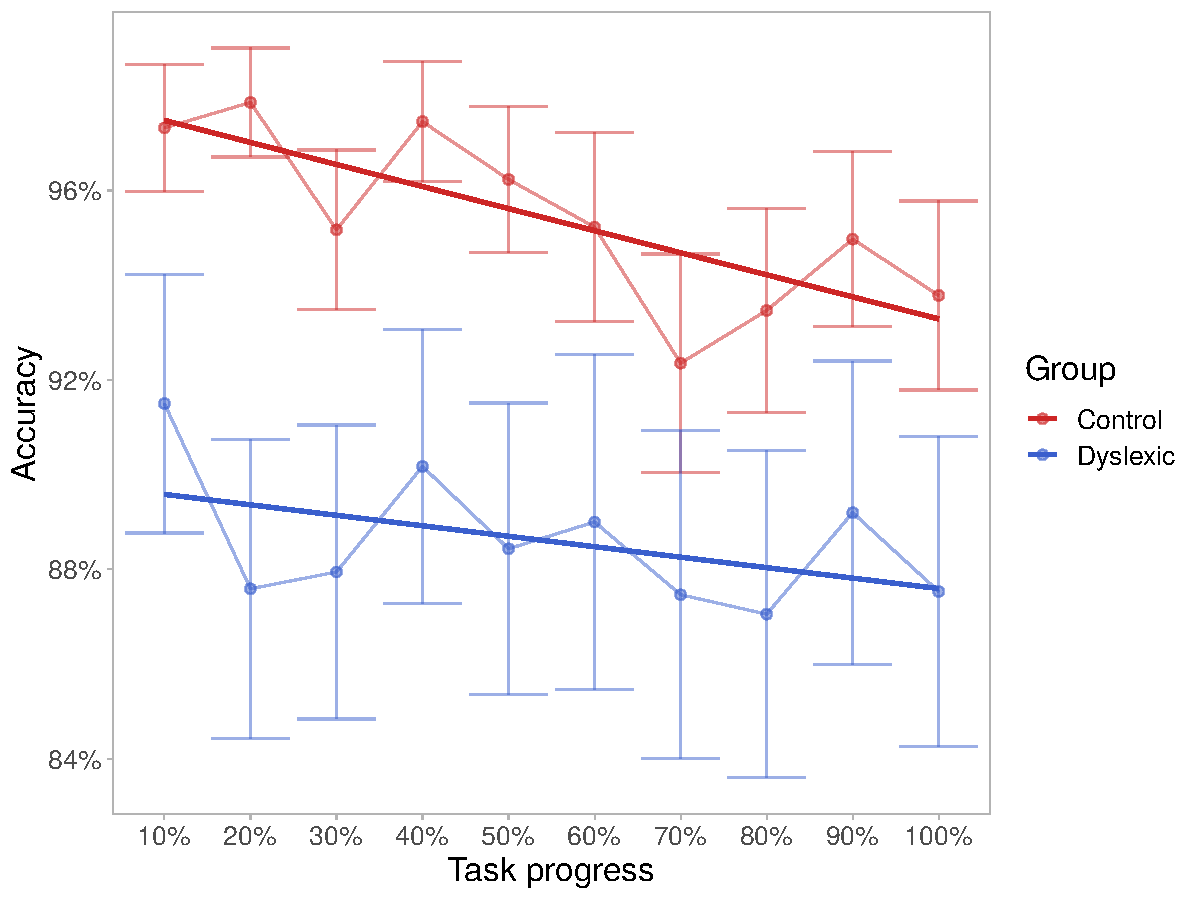
\includegraphics[width = 10 cm]{images/paper_4/fatigue_fx_group.pdf}
    \item \textit{Each point represents the average accuracy within a group in a certain interval of the task. Error bars mark the 95\% confidence interval  of the mean. The x-axis marks progress through the task: 10\% marks the first 21 of 210 trials, 20\% marks trials 22-42, and so on. Dark lines indicate the best fit regression line.}
\end{figure}

\section{Discussion}
We considered how the frequency distribution from which stimuli are drawn during a standard phoneme labeling task might deferentially affect task-performance in children with dyslexia versus typical readers. Indeed, some authors have posited that differences in psychophysical task performance may, in some situations, actually reflect a difference in an individual's sensitivity to task conditions (i.e., the distribution of the stimuli). Because our task did not appear to induce measurable statistical learning effects in participants of any reading ability, we are unable to comment on how such effects may differ in children with dyslexia. However, our results replicate many previous findings in our lab and others about the relationship between reading skill and categorical labeling, and suggest that poor readers' behavior on the task is not strongly sensitive to the stimulus frequency distributions.

There are several reasons why we may not have seen clear effects of stimulus distribution, whereas other experimenters have in similar contexts \citep{Vandermosten2018StatisticalChildren,Clayards2008PerceptionCues}: unlike in Vandermosten et al.'s study of distributional learning in children with and without reading disability \citep{Vandermosten2018StatisticalChildren}, we used a native-language contrast that may have been over-learned by our participants prior to our study. If this explanation were true, it would imply that children with dyslexia are entirely equipped to leverage statistical learning to establish phonetic categories from their natural environment (albeit, perhaps to a lesser degree than their typically developing peers). Another explanation is that our measurements may not have been sufficiently precise: Clayards et al. detected stimulus distribution effects on psychometric function shape for a native-language contrast \citep{Clayards2008PerceptionCues}, but used eye-tracking to recover a time-series measure of looks to a closed set of choices displayed on a screen. 

Our data set also allowed us to apply the modeling approach of Lieder et al. \citep{Lieder2019PerceptualDyslexia} to investigate how previous stimulus presentations affect judgments about the current stimulus. We were able to detect effects of the previous two stimulus presentations, but critically, did not find that these effects interacted with reading skill. Our results are broadly consistent with Lieder et al.'s findings, which showed that stimulus recency effects were similar in adults with and without dyslexia (albeit in a task involving the judgment of tone frequency differences). For stimulus recency effects to be intact in children with dylsexia, it seems necessary to also have intact sensory encoding---if stimuli were not encoded with sufficiently high fidelity, it is difficult to imagine that children would be sensitive to differences between previous and current presentations. If our inference is valid, then our results may provide further evidence against the position that less categorical behavior on the phoneme labeling task is a consequence of impaired or noisier sensory processing in poor readers \citep{Goswami2011,Hancock2017NeuralDyslexia,Casini2018ItsDyslexia}. Our results also seem to contradict claims that adaptation or anchoring to recent stimuli is somehow different in children with dyslexia \citep{Jaffe-Dax2017DyslexicsAdaptation,Ahissar2006,Perrachione2016DysfunctionDyslexia,Krause2015PayDyslexia,Nicolson2018ProceduralCommitment}.

Finally, we tested whether children with dyslexia showed signs of increased fatigue during the task by analyzing their performance on relatively easy trials throughout the course of the task. Although individuals with dyslexia showed a tendency to make more errors on "easy" trials throughout the experiment, we did not find evidence to suggest that they were merely becoming less attentive over time, as Messaoud-Galusi et al. did in a similar task \citep{Messaoud-Galusi2011}. It is possible that our results differ because we allowed children a brief break (typically less than one minute) every 35 trials, whereas participants in Messaoud-Galusi and colleague's study adhered to a different schedule. Additionally, our participant demographics may have differed, as many of our children are well-accustomed to computer games at home and at school. While we are therefore cautious to generalize our results broadly, we can conclude that task fatigue is unlikely to explain the patterns of categorical labeling we present here. This may be reassuring with regard to the large literature on categorical labeling in individuals with dyslexia: while experimenters must remain vigilant of ways that overall decreased accuracy can bias measures of task performance \citep{Wichmann2001,Roach2004}, our results suggest that a simple explanation of task engagement alone is unlikely to account for the entire relationship between reading and categorical labeling. 

Considering our results and the current state of the field, we believe researchers are at an intriguing moment: there is compelling evidence that in certain experiments, apparent deficits in groups of participants with dyslexia are well-explained by non-linguistic and non-sensory mechanisms \citep{Gabay2015,Banai2004,Banai2006}, and this framework has considerably more power to explain the diversity of deficits associated with reading disability than purely sensory or phonological models. Still, there are considerable gaps in this explanation: not only are there are experimental contexts where individuals with dyslexia appear to have no statistical learning deficit \citep{Gabay2018,Staels2015NoDyslexia,Gould1990DoDeficit,Inacio2018ImplicitChildren,Jimenez-Fernandez2011DyslexicCueing,Samara2017ArtificialLearning,Du2013ImplicitInformation} (perhaps reflecting ongoing vagueness in what "statistical learning" encompasses), but effect sizes in studies that do detect group differences are too small to accurately separate most cases of dyslexia from typical reading \citep{Lieder2019PerceptualDyslexia,Vandermosten2018StatisticalChildren}. 

Even if we take the view that reduced categorical labeling in struggling readers is entirely the consequence of impaired sensitivity to phonetic categories over the course of many years of language exposure, group separability would remain quite modest: the average effect size in categorical labeling studies is 0.66 \citep{Noordenbos2015}, meaning that only 9.7\% of individuals with dyslexia would fall below the 95\% confidence interval of the control population. A further problem for the statistical learning hypothesis is that it often relies on an assumption that a very subtle impairment can cascade to have drastic effects on literacy by disrupting the development of typical phonological processing. However, our previous studies \citep{OBrien2018,OBrien2019CategoricalDuration} and several others \citep{Robertson2009,Snowling2019LongitudinalDyslexia,Talcott2000,Calcus2018} suggest that a cascading model is inadequate: performance on psychophysical tasks can relate to reading skill separately from the proposed phonological processing mediation pathway. It may be that the categorical labeling task is an index of something far broader than phonological awareness, such as overall developmental status or linguistic experience. Sharpening of category boundaries may be partially a result of reading experience itself.

In sum, our results are consistent with the perspective that multiple causal routes relate performance on various behavioral and psychophysical measures to reading skill \citep{Pennington2012IndividualModels.,Ziegler2019ModelingDyslexia}. Under this model, deficits in learning category boundaries from speech sounds may be one of many factors that contribute to difficulties with reading. In light of this, we are most optimistic towards future research that explores how constellations of risk factors, including but not limited to reduced category learning, phonological processing, and sensitivity to the statistics of non-linguistic stimuli, act in concert to determine a child's reading skill. 




\end{document}